\newcommand{\scale}{2}
\section{Komposition}
\lettrine{K}{omposition} zur Anordnung von Bildteilung in Flächen.

\subsection{Flächenaufteilung}
\begin{multicols}{2}
\begin{minipage}{3cm}
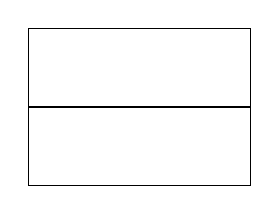
\begin{tikzpicture}[scale=\scale]
	\draw (0,0) -- (1.41,0) -- (1.41,1) --(0,1) -- (0,0);
	\draw (0,0.5) -- (1.41,0.5);
\end{tikzpicture}
\end{minipage}
\begin{minipage}{5cm}
\begin{itemize}
	\item liegend
	\item Ruhe
\end{itemize}
\end{minipage}

\vspace{0.2cm}

\begin{minipage}{2.3cm}
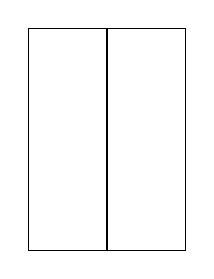
\begin{tikzpicture}[scale=\scale]
	\draw (0,0) -- (1,0) -- (1,1.41) --(0,1.41) -- (0,0);
	\draw (0.5,0) -- (0.5,1.41);
\end{tikzpicture}
\end{minipage}
\begin{minipage}{5cm}
\begin{itemize}
	\item stehend
	\item Wachheit
	\item ein Gegenüber
\end{itemize}
\end{minipage}

\vspace{0.2cm}

\begin{minipage}{2.3cm}
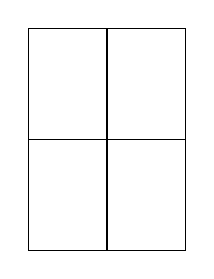
\begin{tikzpicture}[scale=\scale]
	\draw (0,0) -- (1,0) -- (1,1.41) --(0,1.41) -- (0,0);
	\draw (0.5,0) -- (0.5,1.41);
	\draw (0,0.705) -- (1,0.705);
\end{tikzpicture}
\end{minipage}
\begin{minipage}{5cm}
\begin{itemize}
	\item Ausgleich
\end{itemize}
\end{minipage}

\vspace{0.2cm}

\begin{minipage}{2.3cm}
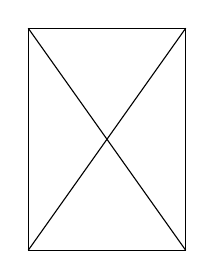
\begin{tikzpicture}[scale=\scale]
	\draw (0,0) -- (1,0) -- (1,1.41) --(0,1.41) -- (0,0);
	\draw (0,0) -- (1,1.41);
	\draw (1,0) -- (0,1.41);
\end{tikzpicture}
\end{minipage}
\begin{minipage}{5cm}
\begin{itemize}
	\item Zentrierung
\end{itemize}
\end{minipage}

\begin{minipage}{2.3cm}
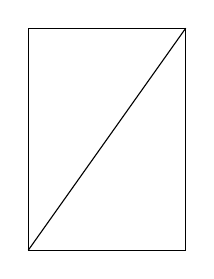
\begin{tikzpicture}[scale=\scale]
	\draw (0,0) -- (1,0) -- (1,1.41) --(0,1.41) -- (0,0);
	\draw (0,0) -- (1,1.41);
\end{tikzpicture}

\vspace{0.1cm}

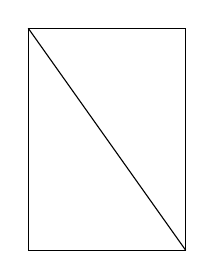
\begin{tikzpicture}[scale=\scale]
	\draw (0,0) -- (1,0) -- (1,1.41) --(0,1.41) -- (0,0);
	\draw (1,0) -- (0,1.41);
\end{tikzpicture}
\end{minipage}
\begin{minipage}{5cm}
\begin{itemize}
	\item Bewegung
	\item Strebt nach außen
\end{itemize}
\end{minipage}

\vspace{0.2cm}

\begin{minipage}{2.3cm}
\begin{tikzpicture}[scale=\scale]
	\draw (0,0) -- (1,0) -- (1,1.41) --(0,1.41) -- (0,0);
	\draw (0,1.1) -- (1,1.1);
\end{tikzpicture}
\end{minipage}
\begin{minipage}{5cm}
\begin{itemize}
	\item Asymmetrie
	\item Spannung
\end{itemize}
\end{minipage}

\begin{minipage}{3cm}
\begin{tikzpicture}[scale=\scale]
	\draw (0,0) -- (1.41,0) -- (1.41,1) --(0,1) -- (0,0);
	\draw (0,0.618) -- (1.41,0.618);
\end{tikzpicture}
\end{minipage}
\begin{minipage}{5cm}
\begin{itemize}
	\item Goldener Schnitt
	\item Harmonisch
	\item $\frac{M}{m}=\frac{\overline{AB}}{\overline{AS}}$
\end{itemize}
\end{minipage}
\end{multicols}

\subsection{Ordnungsprinzipien}
\begin{multicols}{2}
\begin{minipage}{3cm}
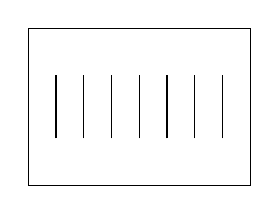
\begin{tikzpicture}[scale=\scale]
	\draw (0,0) -- (1.41,0) -- (1.41,1) --(0,1) -- (0,0);
	\foreach \x in {0.17625,0.3525,...,1.23375}{
	  \draw (\x,0.3) -- (\x,0.7);
	}
\end{tikzpicture}
\end{minipage}
\begin{minipage}{5cm}
\begin{itemize}
	\item Reihung
	\item Ordnung
\end{itemize}
\end{minipage}

\vspace{0.2cm}

\newcount\xb
\newcount\xa
\newcount\xc
\newcount\ya
\newcount\yb
\newcommand{\genrandy}{\setrannum{\ya}{1}{4}\setrannum{\yb}{5}{7}}
\begin{minipage}{3cm}
\begin{tikzpicture}[scale=\scale]
	\draw (0,0) -- (1.41,0) -- (1.41,1) --(0,1) -- (0,0);
	\xb=0
	\foreach \x in {1,2,...,18}{
	  \setrannum{\xa}{1}{6}\setrannum{\xc}{1}{9}\genrandy
	  \draw (\the\xb.\the\xa\the\xc\x,0.\the\ya\x) -- (\the\xb.\the\xa\the\xc\x,0.\the\yb\x);
	}
	\xb=1
	\foreach \x in {1,2,...,12}{
	  \setrannum{\xa}{0}{3}\setrannum{\xc}{1}{9}\genrandy
	  \draw (\the\xb.\the\xa\the\xc\x,0.\the\ya\x) -- (\the\xb.\the\xa\the\xc\x,0.\the\yb\x);
	}
\end{tikzpicture}
\end{minipage}
\begin{minipage}{5cm}
\begin{itemize}
	\item Gruppierung
	\item Spannung
\end{itemize}
\end{minipage}

\renewcommand{\genrandy}{\setrannum{\ya}{1}{4}\setrannum{\yb}{5}{9}}
\begin{minipage}{3cm}
\begin{tikzpicture}[scale=\scale]
	\draw (0,0) -- (1.41,0) -- (1.41,1) --(0,1) -- (0,0);
	\xb=0
	\foreach \x in {1,2,...,15}{
	  \setrannum{\xa}{2}{5}\setrannum{\xc}{1}{9}\genrandy
	  \draw (\the\xb.\the\xa\the\xc\x,0.\the\ya\x) -- (\the\xb.\the\xa\the\xc\x,0.\the\yb\x);
	}
\end{tikzpicture}
\end{minipage}
\begin{minipage}{5cm}
\begin{itemize}
	\item Ballung
	\item Blickfang
\end{itemize}
\end{minipage}

\vspace{0.2cm}

\newcount\xe
\renewcommand{\genrandy}{\setrannum{\ya}{1}{4}\setrannum{\yb}{5}{8}
\setrannum{\temp}{1}{4}
\ifthenelse{\equal{\the\temp}{1}}{\advance\xa by 3}{}
\ifthenelse{\equal{\the\temp}{2}}{\advance\xe by 3}{}
\ifthenelse{\equal{\the\temp}{3}}{\advance\xa by 1}{}
\ifthenelse{\equal{\the\temp}{4}}{\advance\xe by 1}{}
\temp=0
}
\begin{minipage}{3cm}
\begin{tikzpicture}[scale=\scale]
	\draw (0,0) -- (1.41,0) -- (1.41,1) --(0,1) -- (0,0);
	\xb=0
	\foreach \x in {1,2,...,12}{
	  \setrannum{\xa}{1}{9}\setrannum{\xc}{1}{9}\setrannum{\xe}{2}{5}\genrandy
	  \draw (\the\xb.\the\xa\the\xc\x,0.\the\ya\x) -- (\the\xb.\the\xe\the\xa\the\xc\x,0.\the\yb\x);
	}
	\xb=1
	\foreach \x in {1,2,...,6}{
	  \setrannum{\xa}{0}{1}\setrannum{\xc}{1}{5}\setrannum{\xe}{0}{1}\genrandy
	  \draw (\the\temp.\the\xa\the\xc\x,0.\the\ya\x) -- (\the\xb.\the\xe\the\xa\the\xc\x,0.\the\yb\x);
	}
\end{tikzpicture}
\end{minipage}
\begin{minipage}{5cm}
\begin{itemize}
	\item Steuerung
	\item Chaos
\end{itemize}
\end{minipage}
\end{multicols}
